\documentclass{article}
%==============================================================================%
%                                 Packages                                     %
%==============================================================================%
% Packages
\usepackage[utf8]{inputenc}
\usepackage{graphicx}
\usepackage{float}
\usepackage{amsmath}
\usepackage{amssymb}
\usepackage{braket}
\usepackage{subcaption}
\usepackage[margin=0.7in]{geometry}
\usepackage[version=4]{mhchem}
%==============================================================================%
%                           User-Defined Commands                              %
%==============================================================================%
% User-Defined Commands
\newcommand{\be}{\begin{equation}}
\newcommand{\ee}{\end{equation}}
\newcommand{\benum}{\begin{enumerate}}
\newcommand{\eenum}{\end{enumerate}}
\newcommand{\pd}{\partial}
\newcommand{\dg}{\dagger}
\newcommand{\ha}{\hat{A}}
\newcommand{\hb}{\hat{B}}
\newcommand{\hc}{\hat{C}}
%==============================================================================%
%                             Title Information                                %
%==============================================================================%
\title{Position Autocorrelation Function for a Harmonic Oscillator}
\date{\today}
\author{Alan Robledo}
\begin{document}
\maketitle
\section{Theory}
\subsection{Canonical ensemble}
As always we define the Hamiltonian for the 1D system.
\be
  H = \frac{p^2}{2m} + \frac{1}{2} m \omega^2 x^2
\ee
In the canonical ensemble, $C_{xx}(t)$ for a 1D Harmonic Oscillator has a simple form,
\be
  C_{xx}(t) = \frac{kT}{m \omega^2} \cos(\omega t)
\ee
where $k$ is Boltzmann's constant and $T$ is temperature. Computing this value numerically with a single Molecular Dynamics trajectory poses an issue because the correlation function requires that the dynamics be realistic --- something that cannot be generated for a system coupled to a thermal bath. We can overcome this issue by defining the correlation function in the microcanonical ensemble.

\subsection{Microcanonical ensemble}
The first thing we need to do is compute the partition function for a Harmonic Oscillator in the microcanonical ensemble, i.e. we need to compute,
\be
  \begin{split}
    \Omega &= \frac{E_o}{h} \int_{-\infty}^{\infty} dp \int_{-\infty}^{\infty} dx \; \delta(H(x,p) - E) \\
    &= \frac{E_o}{h} \int_{-\infty}^{\infty} dp \int_{-\infty}^{\infty} dx \; \delta\left( \frac{p^2}{2m} + \frac{1}{2} m \omega^2 x^2 - E \right)
  \end{split}
\ee
which is non-trivial but doable. We begin by defining some new coordinates,
\be \label{eq:bar_coords}
  \begin{split}
    \bar{p} &= \frac{p}{\sqrt{2m}} \quad ; \quad \sqrt{2m} d\bar{p} = dp \\
    \bar{x} &= \sqrt{ \frac{m \omega^2}{2} } x \quad ; \quad \sqrt{ \frac{2}{m \omega^2} } d\bar{x} = dx
  \end{split}
\ee
and substituting them into the partition function.
\be
  \begin{split}
    \Omega &= \frac{E_o}{h} \sqrt{2m} \sqrt{ \frac{2}{m \omega^2} } \int_{-\infty}^{\infty} d \bar{p} \int_{-\infty}^{\infty} d\bar{x} \; \delta\left( \bar{p}^2 +  \bar{x}^2 - E \right) \\
    &= \frac{2 E_o}{h \omega} \int_{-\infty}^{\infty} d \bar{p} \int_{-\infty}^{\infty} d\bar{x} \; \delta\left( \bar{p}^2 + \bar{x}^2 - E \right)
  \end{split}
\ee
The delta function requires that we consider points where $p^2 + x^2 = E$ which resembles the equation for a circle so we can consider a conversion to polar coordinates.
\be \label{eq:polar_coords}
  \begin{split}
    \bar{p} &= \sqrt{r \omega} \cos(\theta) \\
    \bar{x} &= \sqrt{r \omega} \sin(\theta)
  \end{split}
\ee
We define the coordinates this way so that the jacobian is simply a factor of $\omega$.
\be
  |J| =
  \begin{vmatrix}
    \frac{\partial \bar{p}}{\partial r} & \frac{\partial \bar{p}}{\partial \theta}\\[6pt]
    \frac{\partial \bar{x}}{\partial r} & \frac{\partial \bar{x}}{\partial \theta}
  \end{vmatrix}
  =
  \begin{vmatrix}
    \sqrt{\omega} \cos(\theta) / 2\sqrt{r} & - \sqrt{r \omega} \sin(\theta) \\
    \sqrt{\omega} \sin(\theta) / 2\sqrt{r} & \sqrt{r \omega} \cos(\theta) \\
  \end{vmatrix}
  = \frac{\omega}{2} \cos^2(\theta) + \frac{\omega}{2} \sin^2(\theta) = \frac{\omega}{2}
\ee
The integrals become redefined as,
\be
  \int_{-\infty}^{\infty} d \bar{p} \int_{-\infty}^{\infty} d\bar{x} = \int_{0}^{2 \pi} d \theta \int_{0}^{\infty} d r |J|  = \frac{\omega}{2} \int_{0}^{2 \pi} d \theta \int_{0}^{\infty} d r
\ee
Equation (5) becomes,
\be
  \Omega = \frac{E_o}{h} \int_{0}^{2 \pi} d \theta \int_{0}^{\infty} d r \; \delta\left( r \omega - E \right)
\ee
The integral over $\theta$ is trivial,
\be
  \Omega = \frac{2 \pi E_o}{h} \int_{0}^{\infty} d r \; \delta\left( r \omega - E \right)
\ee
and we can set $r' = r \omega$,
\be
  \Omega = \frac{2 \pi E_o}{h \omega} \int_{0}^{\infty} d r' \; \delta\left( r' - E \right)
\ee
to get an integral of a dirac delta function over all space which is equal to 1. So we are left with,
\be
  \Omega = \frac{2 \pi E_o}{h \omega} = \frac{E_o}{\hbar \omega} .
\ee

Now we can begin deriving a form for the correlation function.
We start with the definition of $C_{xx}(t)$ in the microcanonical ensemble (we take $t=0$ to be our initial time) as a phase space average,
\be
  C_{xx}(t) = \braket{x(0) x(t)} = \frac{E_o}{h \Omega} \int_{-\infty}^{\infty} dp \int_{-\infty}^{\infty} dx \; x(0) \; x(t) \delta(H(x,p) - E)
\ee
where $E_o/h$ is a constant from the partition function $\Omega$.
Integrating Hamilton's equations for a Harmonic Oscillator yields the equation of motion
\be
  x(t) = x(0) \cos(\omega t) + \frac{p(0)}{m \omega} \sin(\omega t)
\ee
where $p(0)$ is the initial momentum. We can drop the 0 in the initial x and p since we need to consider each point in phase space as an initial condition in order to compute the integral. Plugging $x(t)$ and equation (12) into our defintion leaves us with,
\be
  C_{xx}(t) = \frac{\omega}{2 \pi} \int_{-\infty}^{\infty} dp \int_{-\infty}^{\infty} dx \; x \left[ x \cos(\omega t) + \frac{p}{m \omega} \sin(\omega t) \right] \delta \left( \frac{p^2}{2m} + \frac{1}{2} m \omega^2 x^2 - E \right)
\ee
We will now make the same transformation as in equation (\ref{eq:bar_coords}) to make $(x,p) \rightarrow (\bar{x}, \bar{p})$.
\be
\begin{split}
  C_{xx}(t) &= \frac{\omega}{2 \pi} \sqrt{2m} \sqrt{ \frac{2}{m \omega^2} } \int_{-\infty}^{\infty} d \bar{p} \int_{-\infty}^{\infty} d \bar{x} \; \sqrt{\frac{2}{m \omega^2}} \bar{x} \left[ \sqrt{\frac{2}{m \omega^2}} \bar{x} \cos(\omega t) + \frac{\sqrt{2m}}{m \omega} \bar{p} \sin(\omega t) \right] \delta \left( \bar{p}^2 + \bar{x}^2 - E \right) \\
  &= \frac{\omega}{2 \pi} \frac{2}{\omega} \int_{-\infty}^{\infty} d \bar{p} \int_{-\infty}^{\infty} d \bar{x} \; \sqrt{\frac{2}{m \omega^2}} \bar{x} \left[ \sqrt{\frac{2}{m \omega^2}} \bar{x} \cos(\omega t) + \sqrt{\frac{2}{m \omega^2}} \bar{p} \sin(\omega t) \right] \delta \left( \bar{p}^2 + \bar{x}^2 - E \right) \\
  &= \frac{1}{\pi} \int_{-\infty}^{\infty} d \bar{p} \int_{-\infty}^{\infty} d \bar{x} \; \frac{2}{m \omega^2} \bar{x} \left[ \bar{x} \cos(\omega t) + \bar{p} \sin(\omega t) \right] \delta \left( \bar{p}^2 + \bar{x}^2 - E \right) \\
  &= \frac{2}{ \pi m \omega^2} \int_{-\infty}^{\infty} d \bar{p} \int_{-\infty}^{\infty} d \bar{x} \; \bar{x} \left[ \bar{x} \cos(\omega t) + \bar{p} \sin(\omega t) \right] \delta \left( \bar{p}^2 + \bar{x}^2 - E \right) \\
\end{split}
\ee
And then make the second transformation to polar coordinates as in equation (\ref{eq:polar_coords}).
\be
  \begin{split}
    C_{xx}(t) &= \frac{2}{ \pi m \omega^2} \frac{\omega}{2} \int_{0}^{2 \pi} d \theta \int_{0}^{\infty} d r \; \sqrt{r \omega} \sin(\theta) \left[ \sqrt{r \omega} \sin(\theta) \cos(\omega t) + \sqrt{r \omega} \cos(\theta) \sin(\omega t) \right] \delta \left( r \omega - E \right) \\
    &= \frac{1}{ \pi m \omega} \int_{0}^{2 \pi} d \theta \int_{0}^{\infty} d r \; r \omega \sin(\theta) \left[ \sin(\theta) \cos(\omega t) + \cos(\theta) \sin(\omega t) \right] \delta \left( r \omega - E \right) \\
  \end{split}
\ee
The following trig identity, $\sin(x)\cos(y) + \sin(y)\cos(x) = \sin(x+y)$, yields,
\be
\begin{split}
  C_{xx}(t) &= \frac{1}{ \pi m} \int_{0}^{2 \pi} d \theta \int_{0}^{\infty} d r \; r \sin(\theta) \left[ \sin(\theta + \omega t) \right] \delta \left( r \omega - E \right) \\
  &= \frac{1}{ \pi m} \int_{0}^{\infty} d r \; r \; \delta \left( r \omega - E \right) \int_{0}^{2 \pi} d \theta \sin(\theta) \sin(\theta + \omega t)
\end{split}
\ee
The theta integral is trivial.
\be
\begin{split}
  \int_{0}^{2 \pi} d \theta \sin(\theta) \sin(\theta + \omega t) &= \int_{0}^{2 \pi} d \theta \sin(\theta) \left[ \sin(\theta) \cos(\omega t) + \cos(\theta) \sin(\omega t) \right] \\
  &= \cos(\omega t) \int_{0}^{2 \pi} d \theta \sin^2 (\theta) + \sin(\omega t) \int_{0}^{2 \pi} d \theta \sin(\theta) \cos(\theta) \\
  &= \cos(\omega t) \int_{0}^{2 \pi} d \theta \frac{1}{2} \left[ 1 - \cos(2 \theta)\right] + \sin(\omega t) \int_{0}^{2 \pi} d \theta \sin(\theta) \cos(\theta) \\
  &= \frac{\cos(\omega t)}{2} \int_{0}^{2 \pi} d \theta \left[ 1 - \cos(2 \theta)\right] + \sin(\omega t) \int_{0}^{0} du \; u \\
  &= \frac{\cos(\omega t)}{2} \left( \theta - \frac{\sin(2 \theta)}{2} \right) \bigg|^{2 \pi}_0 + 0\\
  &= \frac{\cos(\omega t)}{2} (2\pi) \\
  &= \pi \cos(\omega t)
\end{split}
\ee
So we are left with,
\be
  C_{xx}(t) = \frac{1}{m} \int_{0}^{\infty} d r \; r \cos(\omega t) \delta \left( r \omega - E \right)
\ee
If we set $r' = r \omega$ we are left with another delta function that is simple to evaluate with the following identity, $\int_{-\infty}^{\infty} f(x) \delta(x - a) = f(a)$, (remembering that $r \in [0, \infty)$)
\be
\begin{split}
  C_{xx}(t) &= \frac{1}{m} \int_{0}^{\infty} \frac{d r'}{\omega} \; \frac{r'}{\omega} \cos(\omega t) \delta \left( r' - E \right) \\
  &= \frac{1}{m \omega^2} \cos(\omega t) \int_{0}^{\infty} dr' \; r' \delta \left( r' - E \right) \\
  &= \frac{1}{m \omega^2} \cos(\omega t) E
\end{split}
\ee
And we finally derive the position autocorrelation function in the microcanonical ensemble,
\be
  C_{xx}(t) = \frac{E}{m \omega^2} \cos(\omega t)
\ee
where $E$ is the constant total energy of the system.

\section{Code results}
The code '1dharmonic.py' defines a Harmonic Oscillator with mass $m=3$ and frequency $\omega = 2$. Thefore, $E = \frac{3}{2} v^2 + 6 x^2$. A single trajectory is generated with 50,000 total MD steps and a time step of 0.01. Then the code takes segments of the trajectory of 500 MD steps and computes the correlation function by treating each of the segments as independent trajectories.
\begin{figure}[H]
    \centering
        % height adjusts the size of the photo.
    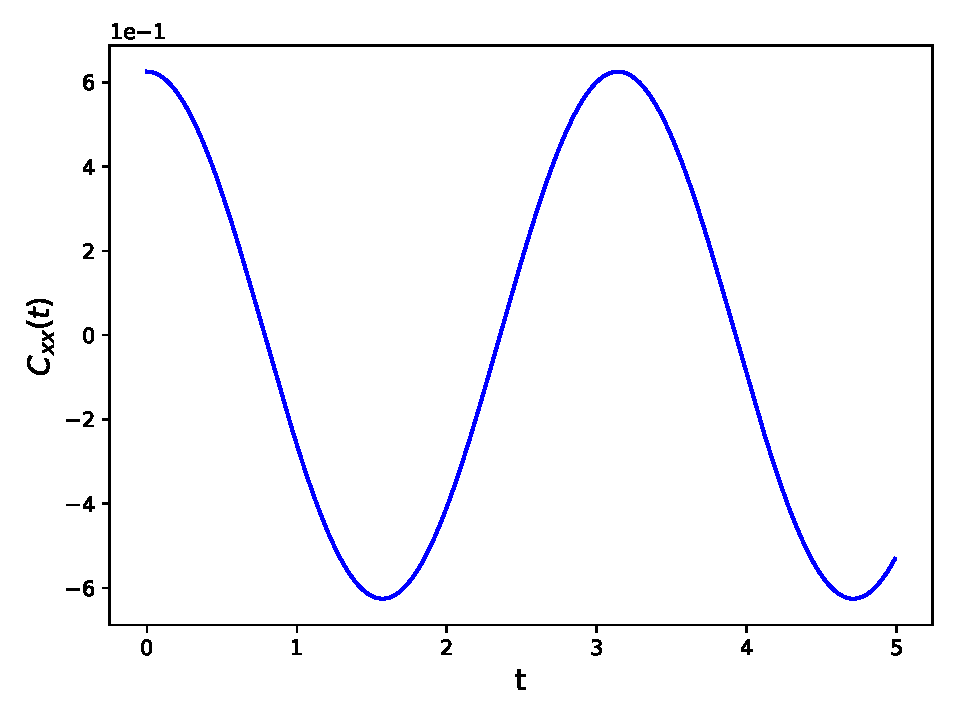
\includegraphics[height=2.6in]{figures/1d_position_auto.pdf}
    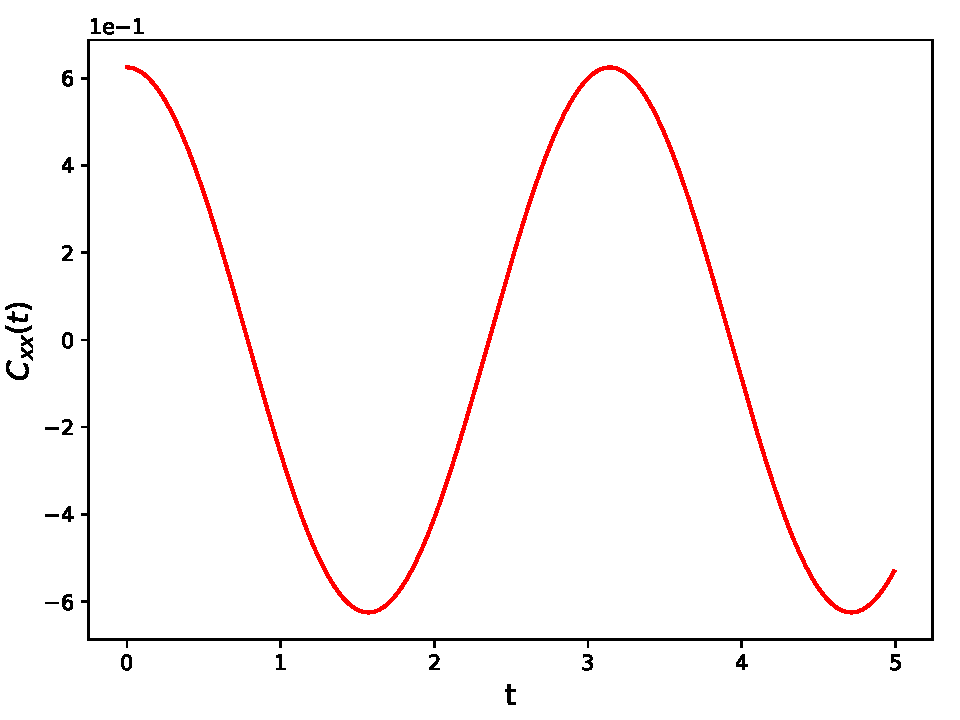
\includegraphics[height=2.6in]{figures/ideal.pdf}
    \caption{(Left) Plot of position autocorrelation over 500 MD steps with a time step of 0.01 computed from a single trajectory with 50,000 total steps. (Right) Plot of position autocorrelation over 500 MD steps with a time step of 0.01 computed using equation (22).}
\end{figure}
\end{document}
